% Created by tikzDevice version 0.8.1 on 2015-06-27 20:39:43
% !TEX encoding = UTF-8 Unicode
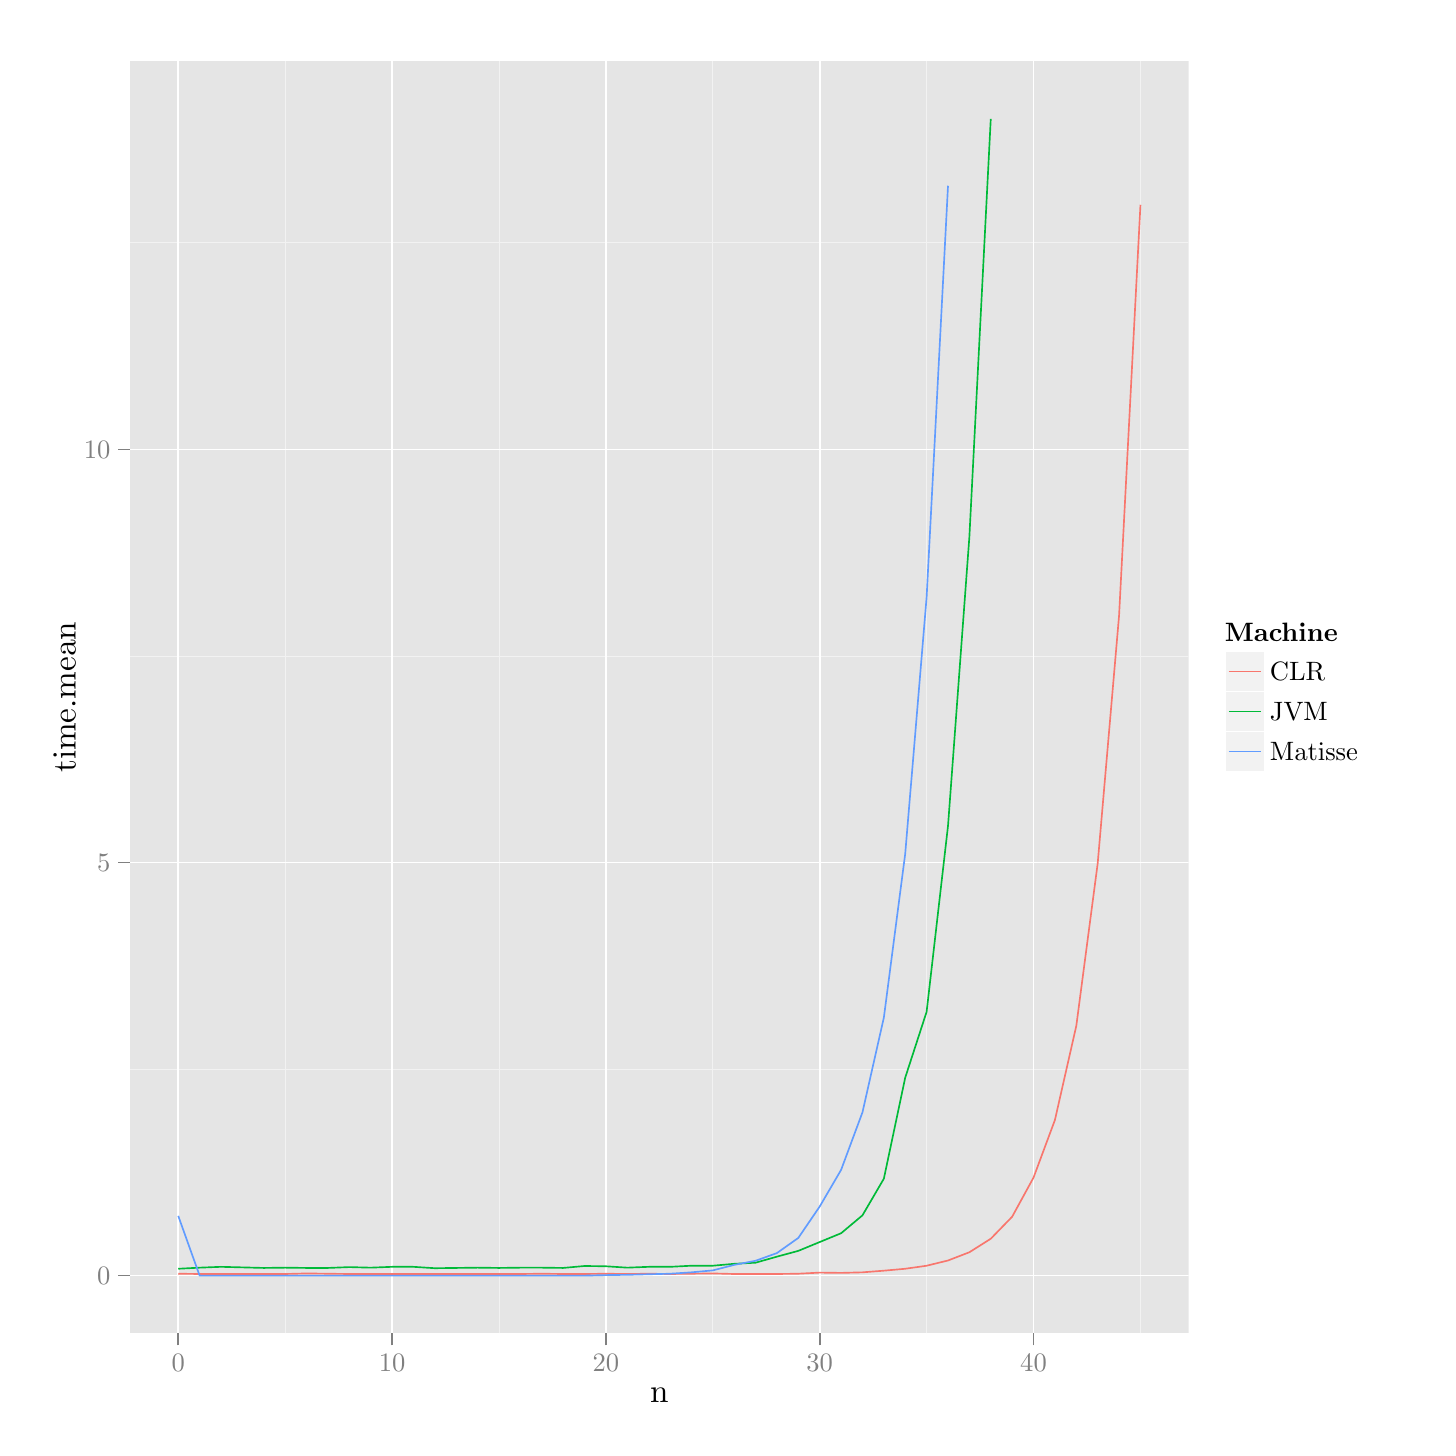
\begin{tikzpicture}[x=1pt,y=1pt]
\definecolor{fillColor}{RGB}{255,255,255}
\path[use as bounding box,fill=fillColor,fill opacity=0.00] (0,0) rectangle (505.89,505.89);
\begin{scope}
\path[clip] (  0.00,  0.00) rectangle (505.89,505.89);
\definecolor{drawColor}{RGB}{255,255,255}
\definecolor{fillColor}{RGB}{255,255,255}

\path[draw=drawColor,line width= 0.6pt,line join=round,line cap=round,fill=fillColor] (  0.00,  0.00) rectangle (505.89,505.89);
\end{scope}
\begin{scope}
\path[clip] ( 37.02, 34.03) rectangle (419.48,493.85);
\definecolor{fillColor}{gray}{0.90}

\path[fill=fillColor] ( 37.02, 34.03) rectangle (419.48,493.85);
\definecolor{drawColor}{gray}{0.95}

\path[draw=drawColor,line width= 0.3pt,line join=round] ( 37.02,129.58) --
	(419.48,129.58);

\path[draw=drawColor,line width= 0.3pt,line join=round] ( 37.02,278.87) --
	(419.48,278.87);

\path[draw=drawColor,line width= 0.3pt,line join=round] ( 37.02,428.16) --
	(419.48,428.16);

\path[draw=drawColor,line width= 0.3pt,line join=round] ( 93.04, 34.03) --
	( 93.04,493.85);

\path[draw=drawColor,line width= 0.3pt,line join=round] (170.30, 34.03) --
	(170.30,493.85);

\path[draw=drawColor,line width= 0.3pt,line join=round] (247.57, 34.03) --
	(247.57,493.85);

\path[draw=drawColor,line width= 0.3pt,line join=round] (324.83, 34.03) --
	(324.83,493.85);

\path[draw=drawColor,line width= 0.3pt,line join=round] (402.10, 34.03) --
	(402.10,493.85);
\definecolor{drawColor}{RGB}{255,255,255}

\path[draw=drawColor,line width= 0.6pt,line join=round] ( 37.02, 54.94) --
	(419.48, 54.94);

\path[draw=drawColor,line width= 0.6pt,line join=round] ( 37.02,204.22) --
	(419.48,204.22);

\path[draw=drawColor,line width= 0.6pt,line join=round] ( 37.02,353.51) --
	(419.48,353.51);

\path[draw=drawColor,line width= 0.6pt,line join=round] ( 54.41, 34.03) --
	( 54.41,493.85);

\path[draw=drawColor,line width= 0.6pt,line join=round] (131.67, 34.03) --
	(131.67,493.85);

\path[draw=drawColor,line width= 0.6pt,line join=round] (208.93, 34.03) --
	(208.93,493.85);

\path[draw=drawColor,line width= 0.6pt,line join=round] (286.20, 34.03) --
	(286.20,493.85);

\path[draw=drawColor,line width= 0.6pt,line join=round] (363.46, 34.03) --
	(363.46,493.85);
\definecolor{drawColor}{RGB}{248,118,109}

\path[draw=drawColor,line width= 0.6pt,line join=round] ( 54.41, 55.63) --
	( 62.13, 55.53) --
	( 69.86, 55.53) --
	( 77.58, 55.53) --
	( 85.31, 55.53) --
	( 93.04, 55.53) --
	(100.76, 55.73) --
	(108.49, 55.63) --
	(116.22, 55.53) --
	(123.94, 55.53) --
	(131.67, 55.53) --
	(139.40, 55.53) --
	(147.12, 55.53) --
	(154.85, 55.53) --
	(162.58, 55.53) --
	(170.30, 55.53) --
	(178.03, 55.53) --
	(185.75, 55.63) --
	(193.48, 55.53) --
	(201.21, 55.53) --
	(208.93, 55.63) --
	(216.66, 55.53) --
	(224.39, 55.63) --
	(232.11, 55.53) --
	(239.84, 55.63) --
	(247.57, 55.73) --
	(255.29, 55.53) --
	(263.02, 55.53) --
	(270.75, 55.53) --
	(278.47, 55.63) --
	(286.20, 56.03) --
	(293.93, 55.93) --
	(301.65, 56.13) --
	(309.38, 56.73) --
	(317.10, 57.42) --
	(324.83, 58.52) --
	(332.56, 60.41) --
	(340.28, 63.39) --
	(348.01, 68.27) --
	(355.74, 76.23) --
	(363.46, 90.37) --
	(371.19,111.17) --
	(378.92,145.21) --
	(386.64,203.83) --
	(394.37,293.40) --
	(402.10,441.89);
\definecolor{drawColor}{RGB}{0,186,56}

\path[draw=drawColor,line width= 0.6pt,line join=round] ( 54.41, 57.42) --
	( 62.13, 57.82) --
	( 69.86, 58.12) --
	( 77.58, 57.92) --
	( 85.31, 57.72) --
	( 93.04, 57.82) --
	(100.76, 57.72) --
	(108.49, 57.72) --
	(116.22, 58.02) --
	(123.94, 57.82) --
	(131.67, 58.12) --
	(139.40, 58.12) --
	(147.12, 57.62) --
	(154.85, 57.72) --
	(162.58, 57.82) --
	(170.30, 57.72) --
	(178.03, 57.82) --
	(185.75, 57.82) --
	(193.48, 57.72) --
	(201.21, 58.42) --
	(208.93, 58.32) --
	(216.66, 57.82) --
	(224.39, 58.12) --
	(232.11, 58.12) --
	(239.84, 58.52) --
	(247.57, 58.52) --
	(255.29, 59.21) --
	(263.02, 59.61) --
	(270.75, 61.80) --
	(278.47, 63.89) --
	(286.20, 67.08) --
	(293.93, 70.26) --
	(301.65, 76.73) --
	(309.38, 89.97) --
	(317.10,126.49) --
	(324.83,150.28) --
	(332.56,217.46) --
	(340.28,321.86) --
	(348.01,472.94);
\definecolor{drawColor}{RGB}{97,156,255}

\path[draw=drawColor,line width= 0.6pt,line join=round] ( 54.41, 76.53) --
	( 62.13, 54.94) --
	( 69.86, 54.94) --
	( 77.58, 54.94) --
	( 85.31, 54.94) --
	( 93.04, 54.94) --
	(100.76, 54.94) --
	(108.49, 54.94) --
	(116.22, 54.94) --
	(123.94, 54.94) --
	(131.67, 54.94) --
	(139.40, 54.94) --
	(147.12, 54.94) --
	(154.85, 54.94) --
	(162.58, 54.94) --
	(170.30, 54.94) --
	(178.03, 54.94) --
	(185.75, 54.94) --
	(193.48, 54.94) --
	(201.21, 54.94) --
	(208.93, 55.13) --
	(216.66, 55.23) --
	(224.39, 55.43) --
	(232.11, 55.63) --
	(239.84, 56.13) --
	(247.57, 56.83) --
	(255.29, 58.82) --
	(263.02, 60.31) --
	(270.75, 63.10) --
	(278.47, 68.57) --
	(286.20, 79.92) --
	(293.93, 93.15) --
	(301.65,113.95) --
	(309.38,148.19) --
	(317.10,207.41) --
	(324.83,300.07) --
	(332.56,448.76);
\end{scope}
\begin{scope}
\path[clip] (  0.00,  0.00) rectangle (505.89,505.89);
\definecolor{drawColor}{gray}{0.50}

\node[text=drawColor,anchor=base east,inner sep=0pt, outer sep=0pt, scale=  0.96] at ( 29.91, 51.63) {0};

\node[text=drawColor,anchor=base east,inner sep=0pt, outer sep=0pt, scale=  0.96] at ( 29.91,200.92) {5};

\node[text=drawColor,anchor=base east,inner sep=0pt, outer sep=0pt, scale=  0.96] at ( 29.91,350.21) {10};
\end{scope}
\begin{scope}
\path[clip] (  0.00,  0.00) rectangle (505.89,505.89);
\definecolor{drawColor}{gray}{0.50}

\path[draw=drawColor,line width= 0.6pt,line join=round] ( 32.75, 54.94) --
	( 37.02, 54.94);

\path[draw=drawColor,line width= 0.6pt,line join=round] ( 32.75,204.22) --
	( 37.02,204.22);

\path[draw=drawColor,line width= 0.6pt,line join=round] ( 32.75,353.51) --
	( 37.02,353.51);
\end{scope}
\begin{scope}
\path[clip] (  0.00,  0.00) rectangle (505.89,505.89);
\definecolor{drawColor}{gray}{0.50}

\path[draw=drawColor,line width= 0.6pt,line join=round] ( 54.41, 29.77) --
	( 54.41, 34.03);

\path[draw=drawColor,line width= 0.6pt,line join=round] (131.67, 29.77) --
	(131.67, 34.03);

\path[draw=drawColor,line width= 0.6pt,line join=round] (208.93, 29.77) --
	(208.93, 34.03);

\path[draw=drawColor,line width= 0.6pt,line join=round] (286.20, 29.77) --
	(286.20, 34.03);

\path[draw=drawColor,line width= 0.6pt,line join=round] (363.46, 29.77) --
	(363.46, 34.03);
\end{scope}
\begin{scope}
\path[clip] (  0.00,  0.00) rectangle (505.89,505.89);
\definecolor{drawColor}{gray}{0.50}

\node[text=drawColor,anchor=base,inner sep=0pt, outer sep=0pt, scale=  0.96] at ( 54.41, 20.31) {0};

\node[text=drawColor,anchor=base,inner sep=0pt, outer sep=0pt, scale=  0.96] at (131.67, 20.31) {10};

\node[text=drawColor,anchor=base,inner sep=0pt, outer sep=0pt, scale=  0.96] at (208.93, 20.31) {20};

\node[text=drawColor,anchor=base,inner sep=0pt, outer sep=0pt, scale=  0.96] at (286.20, 20.31) {30};

\node[text=drawColor,anchor=base,inner sep=0pt, outer sep=0pt, scale=  0.96] at (363.46, 20.31) {40};
\end{scope}
\begin{scope}
\path[clip] (  0.00,  0.00) rectangle (505.89,505.89);
\definecolor{drawColor}{RGB}{0,0,0}

\node[text=drawColor,anchor=base,inner sep=0pt, outer sep=0pt, scale=  1.20] at (228.25,  9.03) {n};
\end{scope}
\begin{scope}
\path[clip] (  0.00,  0.00) rectangle (505.89,505.89);
\definecolor{drawColor}{RGB}{0,0,0}

\node[text=drawColor,rotate= 90.00,anchor=base,inner sep=0pt, outer sep=0pt, scale=  1.20] at ( 17.30,263.94) {time.mean};
\end{scope}
\begin{scope}
\path[clip] (  0.00,  0.00) rectangle (505.89,505.89);
\definecolor{fillColor}{RGB}{255,255,255}

\path[fill=fillColor] (428.35,232.87) rectangle (484.98,295.01);
\end{scope}
\begin{scope}
\path[clip] (  0.00,  0.00) rectangle (505.89,505.89);
\definecolor{drawColor}{RGB}{0,0,0}

\node[text=drawColor,anchor=base west,inner sep=0pt, outer sep=0pt, scale=  0.96] at (432.62,284.11) {\bfseries Machine};
\end{scope}
\begin{scope}
\path[clip] (  0.00,  0.00) rectangle (505.89,505.89);
\definecolor{drawColor}{RGB}{255,255,255}
\definecolor{fillColor}{gray}{0.95}

\path[draw=drawColor,line width= 0.6pt,line join=round,line cap=round,fill=fillColor] (432.62,266.05) rectangle (447.07,280.50);
\end{scope}
\begin{scope}
\path[clip] (  0.00,  0.00) rectangle (505.89,505.89);
\definecolor{drawColor}{RGB}{248,118,109}

\path[draw=drawColor,line width= 0.6pt,line join=round] (434.06,273.27) -- (445.62,273.27);
\end{scope}
\begin{scope}
\path[clip] (  0.00,  0.00) rectangle (505.89,505.89);
\definecolor{drawColor}{RGB}{255,255,255}
\definecolor{fillColor}{gray}{0.95}

\path[draw=drawColor,line width= 0.6pt,line join=round,line cap=round,fill=fillColor] (432.62,251.59) rectangle (447.07,266.05);
\end{scope}
\begin{scope}
\path[clip] (  0.00,  0.00) rectangle (505.89,505.89);
\definecolor{drawColor}{RGB}{0,186,56}

\path[draw=drawColor,line width= 0.6pt,line join=round] (434.06,258.82) -- (445.62,258.82);
\end{scope}
\begin{scope}
\path[clip] (  0.00,  0.00) rectangle (505.89,505.89);
\definecolor{drawColor}{RGB}{255,255,255}
\definecolor{fillColor}{gray}{0.95}

\path[draw=drawColor,line width= 0.6pt,line join=round,line cap=round,fill=fillColor] (432.62,237.14) rectangle (447.07,251.59);
\end{scope}
\begin{scope}
\path[clip] (  0.00,  0.00) rectangle (505.89,505.89);
\definecolor{drawColor}{RGB}{97,156,255}

\path[draw=drawColor,line width= 0.6pt,line join=round] (434.06,244.37) -- (445.62,244.37);
\end{scope}
\begin{scope}
\path[clip] (  0.00,  0.00) rectangle (505.89,505.89);
\definecolor{drawColor}{RGB}{0,0,0}

\node[text=drawColor,anchor=base west,inner sep=0pt, outer sep=0pt, scale=  0.96] at (448.88,269.97) {CLR};
\end{scope}
\begin{scope}
\path[clip] (  0.00,  0.00) rectangle (505.89,505.89);
\definecolor{drawColor}{RGB}{0,0,0}

\node[text=drawColor,anchor=base west,inner sep=0pt, outer sep=0pt, scale=  0.96] at (448.88,255.51) {JVM};
\end{scope}
\begin{scope}
\path[clip] (  0.00,  0.00) rectangle (505.89,505.89);
\definecolor{drawColor}{RGB}{0,0,0}

\node[text=drawColor,anchor=base west,inner sep=0pt, outer sep=0pt, scale=  0.96] at (448.88,241.06) {Matisse};
\end{scope}
\end{tikzpicture}
